\vssub
\subsection{~Spectral partitioning} \label{sub:num_part}
\conthead{APL Wave / XWaves / IMEDS}{B. Tracy}

\noindent
Fig. \ref{fig:partitions} shows an example surface plot of an energy density
spectrum at one grid point at a specific time.  The amount of energy density
at each frequency-direction intersection is shown by this surface.  The
surface is divided into shaded areas or partitions representing energy from
sub-peaks within the spectrum.  Fig. \ref{fig:partitions} shows four
spectral partitions, an area of windsea and three swell trains.  The total
energy represented by this spectrum can be defined by bulk parameters, such as
the significant wave height $H_s$. The shaded areas, called partitions of the
spectrum, show spectral sub-features that give more information about this
grid point's energy situation.  \ws\ has point and field output options
available to provide quantitative descriptions of these individual spectral
partition such as partition wave height, peak period of partition (parabolic
fit), peak wavelength of partition, mean direction of partition, wind-sea
fraction of partition ($W$) using Eq.~(\ref{eq:wsf}), and the number of
partitions.  In the field output, these parameters correspond to spectral partitioned output fields 
\ref{out:first_part} through \ref{out:last_part} and can be found in
\para\ref{sub:outpars}.

Since the two-dimensional spectrum in Fig.~\ref{fig:partitions} looks like a
topological surface, it is logical to apply an image processing partitioning
algorithm that treats the spectral surface like a topographical surface.  The
partitioning shown in Fig.~\ref{fig:partitions} is based on a digital image
processing watershed algorithm \citep{art:VS91} first prototyped by
\cite{pro:HJ04} for the analysis of ocean wave data. 
The US continental divide where everything to the east goes into the Atlantic
Ocean and everything to the west goes into the Pacific Ocean is a typical
example of a watershed line.  The oceans represent minima that determine the
watershed line.  If the spectral surface is inverted, the spectral peaks
become catchments and watershed lines or partition boundaries can be
determined using the \cite{art:VS91} algorithm.  Calculation of parameters for
each spectral partition can then be accomplished and wave system analysis as
described in \cite{art:HP01} can be applied.  \cite{pro:HJ04} and
\cite{tol:Vict06b} used a MATLAB code to apply the \cite{art:VS91}
algorithm\footnote{~Now available as XWaves from
http://www.WaveForceTechnologies.com, replacing the previous APL WAVES
package}.  This code has been transformed to an efficient FORTRAN routine for
use in \ws since version 3.11.  Coding follows the
\cite{art:VS91} paper but incorporates an efficient sort routine (O(n))
discussed in \cite{rep:TTH06}.

\begin{figure} \begin{center}
\epsfig{file=./num/partition1.eps,width=3.8in}
\caption{Surface plot of an energy density spectrum showing spectral
         partitions for windsea and three swell trains.  This is a snapshot of
         hindcasted conditions at Christmas Island (NOAA buoy 51028) at
         12:00~UTC on November 9, 2000.}
         \label{fig:partitions} \botline
\end{center}
\end{figure}





